\section{Probability and Random Process Theory Review}
\framecard{\insertsection}
\subsection{Basic Concepts of Probability Theory}


\begin{frame}{\insertsubsection}

A key concept in the field of pattern recognition is that of \textbf{uncertainty}, that arises from both through noise on measurements, as well as through the finite size of data sets. To find this uncertainty we'll talk about a little of the \textbf{Probability Theory}. Let's begin from a simple example.

\end{frame}

\begin{frame}{\insertsubsection}

\begin{columns}[t]
	\begin{column}{0.45\textwidth}
	\visible<2->{Let's choose a cell in the \autoref{fig:table-probability}. We define the probability of choose a cell in a given column is $p(X = x_i)=c_i/N$, being $N$ the total number of cells and $c_i = \sum_j n_{ij}$.\\}
	
	\vspace{0.5em}

	\visible<3->{We could say that the probability of choose a cell in a given a row is defined as $p(Y = y_j | X = x_i)=n_{ij}/c_i$. \\}	
	
	\vspace{0.5em}
	
	\visible<4->{And so, the probability of choose a cell is defined as $p(X = x_i,Y = y_j)=n_{ij}/N$ .}
	\end{column}
	\begin{column}[T]{0.45\textwidth}
		\begin{figure}
			\visible<1->{
				\label{fig:table-probability}
				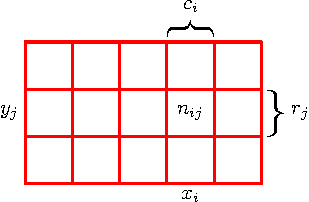
\includegraphics[totalheight=0.4\textheight]{Figure1c10.pdf}
				\caption{Considering in the table $X = x_i$ and $Y = y_j$} }
		\end{figure}
	\end{column}
\end{columns}

\end{frame}

\begin{frame}{\insertsubsection}

Here, we could see some properties that we call \textbf{The Rules of Probability}

\begin{block}{The Rules of Probability}
	\begin{itemize}
		\item Sum Rule: 
		\begin{align} \label{eq:sum-rule}p(X = x_i) =  \sum_j n_{ij} / N
		\visible<2->{ \Rightarrow p(X) = \sum_Y p(X,Y) }
		\end{align}
		\item Product Rule: \begin{align}\label{eq:product-rule}
		p(Y = y_j , X = x_i)=n_{ij}/N \visible<3->{= n_{ij}/c_i \cdot c_i/N}
		\visible<4->{ \Rightarrow p(X,Y) = p(Y|X)p(X) }
\end{align}
\end{itemize}
\end{block}

\end{frame}

\begin{frame}{\insertsubsection}

And by the \textbf{Product Rule} we prove that

\begin{block}{Bayes' Theorem}
\begin{equation}\label{eq:bayes-rule}
	p(X,Y) = p(Y|X)p(X) = p(X|Y)p(Y) \Rightarrow p(Y|X) = \frac{p(X|Y)p(Y)}{p(X)}
\end{equation}
\end{block}

\end{frame}

\begin{frame}{\insertsubsection}

So, from \textbf{The Rules of Probability}, we could show that too 

\begin{block}{Total Probability Theorem}
\begin{equation}\label{eq:total-probability}
	p(X) = \sum_Y p(Y|X)p(X)
\end{equation}
\end{block}

%Remaind of insert the general proof on the appendix

%And so we could derive another formula

%\begin{equation}
%	p(Y|X) = \frac{p(X|Y)p(Y)}{\sum_Y p(Y|X)p(X)}
%\end{equation}

\end{frame}

\begin{frame}{\insertsubsection}

An important propriety of probability is the \textbf{Independence of events}. So, let's say that two events occurs without that one has occurred, so by the \textbf{Bayes' Theorem} we make

\begin{equation}
p(X|Y) = p(X) \text{ and } p(Y|X) = p(Y) \Rightarrow p(X,Y) = p(X)p(Y)
\end{equation}

\end{frame}

\subsection{Random Variables}

\begin{frame}{\insertsubsection}

Simplifying, the \textbf{Random Variables} will treat the probability defined before in the \textit{continuous domain}. So we define a random variable $X$ as a function that assigns a real number, $X(\zeta)$, to each outcome $\zeta$, so $X(\zeta) =  x$.



\end{frame}



\subsection{The Gaussian distribution}
\begin{frame}{\insertsubsection}
The \textbf{Gaussian distribution} is defined as
	\begin{equation}\label{eq:gaussian-distribution}
	\mathcal{N}(x|\mu,\sigma^2) = \frac{1}{(2\pi\sigma^2)^{1/2}}\exp\left\{-\frac{1}{2\sigma^2}(x-\mu)^2\right\}
	\end{equation}
where $\mu$ is the mean and $\sigma^2$ the standard deviation.
\end{frame}


\subsection{Independence of two random variables}
\begin{frame}{\insertsubsection}
\visible<1->{
\begin{block}{Sentence}
\textbf{X and Y are independent random variables} if \textit{any} event $A_1$ defined in terms of $X$ is independent of \textit{any} event $A_2$ defined in terms of Y
\end{block}
}
\visible<2->{
The sentence above is equivalent to say mathematically that
}
\visible<3->{
	\begin{equation}
	P[X \text{ in } A_1, Y \text{ in } A_2]=P[X \text{ in } A_1]P[ Y \text{ in } A_2]
	\end{equation}
}
\visible<4->{
that means in other words that \textit{if $X$ and $Y$ are independent discrete random variables, then the \textbf{joint probability mass function (pmf)} is equal to the product of the marginal pmf's.}
}
\end{frame}

%\begin{frame}{Overleaf users}
%
%\begin{alertblock}{Warning}
%You can ignore this slide if you're \textbf{not} working with Overleaf.
%\end{alertblock}
%
%\vskip 0.5cm
%
%Overleaf, Beamer and Biber do not always get along well together. For this reason, if you make a mistake while writing this presentation, in the drop-down error message you'll \textbf{always} get Biber-related error messages.
%
%\vskip 0.5cm
%
%Luckily, you just have to click on ``\texttt{go to first error/warning}'' and the UI will scroll to the line containing your mistake.
%
%\end{frame}
%
%\begin{frame}[fragile]
%\frametitle{Compiling}
%
%\begin{alertblock}{Warning}
%You can ignore this slide if you're working with Overleaf.
%\end{alertblock}
%
%To compile this deck you'll need the \texttt{biber} package. Probably your \TeX editor already supports it; if not, you will easily find online the instructions to install it.
%
%\vskip 0.5cm
%
%If you're not using an editor, you can compile this presentation using the command line by running:
%
%\begin{verbatim}
%$ pdflatex main.tex
%$ biber main.bcf
%$ pdflatex main.tex
%$ pdflatex main.tex
%\end{verbatim}
%
%
%\end{frame}
